\subsection{Les propositions au client}
\label{subsec:proposals-to-customer}

\paragraph{}
Le logiciel élaboré est le résultat d'un dialogue constant entre le développeur et les acteurs métiers.

Toutes les fonctionnalités implémentées sont issues de propositions de ma part afin de satisfaire les besoins qui me sont soumis.

\paragraph{}
Toutefois, certaines fonctionnalités ont trouvé leur origine dans des propositions spontanées plutôt que dans des discussions.

\paragraph{}
Une première proposition a été de séparer la phase de traitement et la phase de validation.
En effet, seule la phase de traitement existait. 
Lorsque l'on tentait de soumettre un fichier, soit cela réussissait, soit cela échouait et l'on recevait les journaux de l'application\fnmark.
\fntext{Les journaux d'application sont des messages écrits par des développeurs à l'intention d'autres développeurs.}

Une première phase de validation permet de récupérer un rapport de validation.
Une seconde phase, répète la première pour s'assurer de la validité des données, renvoie une erreur en cas d'échec\fnmark, traite les données en cas de réussite et avertit l'utilisateur du succès.
\fntext{Ce n'est pas censé arriver! Le traitement doit être accessible uniquement après le succès de la première phase.}

Ce découpage permet à l'utilisateur de valider son travail au fur et à mesure plutôt que de le soumettre lorsqu'il est complet.
Cela permet de réduire la latence sur le retour d'information et d'encourager les utilisateurs à utiliser l'application.

\paragraph{}
Un second exemple est le flux d'utilisation où j'ai proposé de réduire au maximum le nombre d'opérations.
Pour ce faire, j'ai créé une expérience linéaire où l'action suivante est la seule possible.

\begin{figure}[ht]
    \centering
    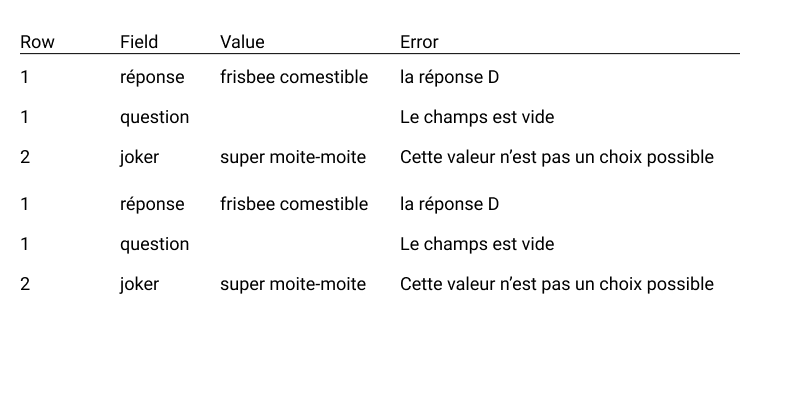
\includegraphics[width=0.7\textwidth]{images/prototypes/spreadsheet-validation.png}
    \caption{Le composant pour visualiser le rapport de validation}
    \label{fig:spreadsheet-validation}
\end{figure}
Ainsi, afin de valider un classeur, observer le succès ou l'échec de la validation, voir le rapport de validation (voir figure \ref{fig:spreadsheet-validation}), soumettre le classeur pour traitement et observer le succès de son traitement, seules deux actions sont requises:
\begin{enumerate}
    \item Glisser et déposer le fichier dans la zone prévue (voir figure \ref{fig:spreadsheet-handler}).
    \item Cliquer sur le bouton prévu pour le traitement.
\end{enumerate}
Cette simplification a pour but d'encourager l'utilisation fréquente de l'application.
\begin{figure}[ht]
    \centering
    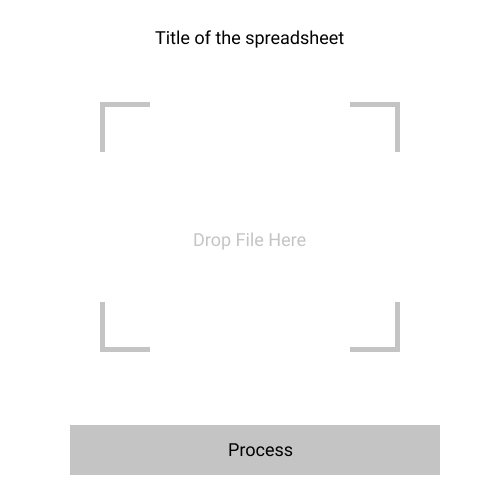
\includegraphics[width=0.7\textwidth]{images/prototypes/spreadsheet-handler.png}
    \caption{Le composant pour recevoir et soumettre les fichiers}
    \label{fig:spreadsheet-handler}
\end{figure}
